% !TeX spellcheck = it_IT

%Controllare anche RFC per studiare
\section{Ad Hoc Distance Vector Routing Protocol AODV}

Ambito WLAN. Si tratta di un \textbf{protocollo di routing}: ha il compito di \textbf{creare e riempire le tabelle di instradamento}. Pensato per una \textbf{rete senza infrastrutture} in cui ogni nodo è anche un router (può fare instradamento). I cammini possono essere multi-hop. I nodi vicini sono quelli nel raggio radio, di conseguenza nodi e vicinati possono variare.\\
I percorsi non vengono creati in modo proattivo: quando serve mandare qualcosa viene richiesto il percorso.\\

Gli \textbf{obiettivi} principali del protocollo sono:
\begin{itemize}
	\item Gestione dinamica della rete ad hoc, ogni nodo può operare secondo protocollo
	\item Auto inizializzante, non sono necessarie rotte preconfigurate; l'inizializzazione deve essere fatta in automatico e periodicamente (per "colpa" della dinamicità della rete)
	\item Loop-free (eliminando il problema del counting to infinity)
	\item Ottenimento di una rotta per una nuova destinazione in tempi rapidi
	\item Risposta rapida alla rottura dei link e al cambio di topologia
\end{itemize}

Le \textbf{funzionalità} che offre sono:
\begin{itemize}
	\item Scoprire e costruire i percorsi per le nuove destinazioni
	\item Mantenere i percorsi in modalità soft-state; ogni percorso ha una durata, se non "rinfrescata" la entry scade e può essere cancellata (eventually)
	\item Riconoscimento errori e cancellazione di percorsi; monitoraggio dell'attività locale e propagazione delle informazioni
\end{itemize}

Si tratta di un protocollo a livello di applicazione (usa UPD 654) che permette di creare tabelle di routing a livello di rete. Ogni nodo è responsabile delle proprie entry, il protocollo è completamente distribuito.\\

\newpage

I dati vengono inviati tra originator e destinazione tramite percorsi simmetrici, non ci sono percorsi indipendenti.
\begin{center}
	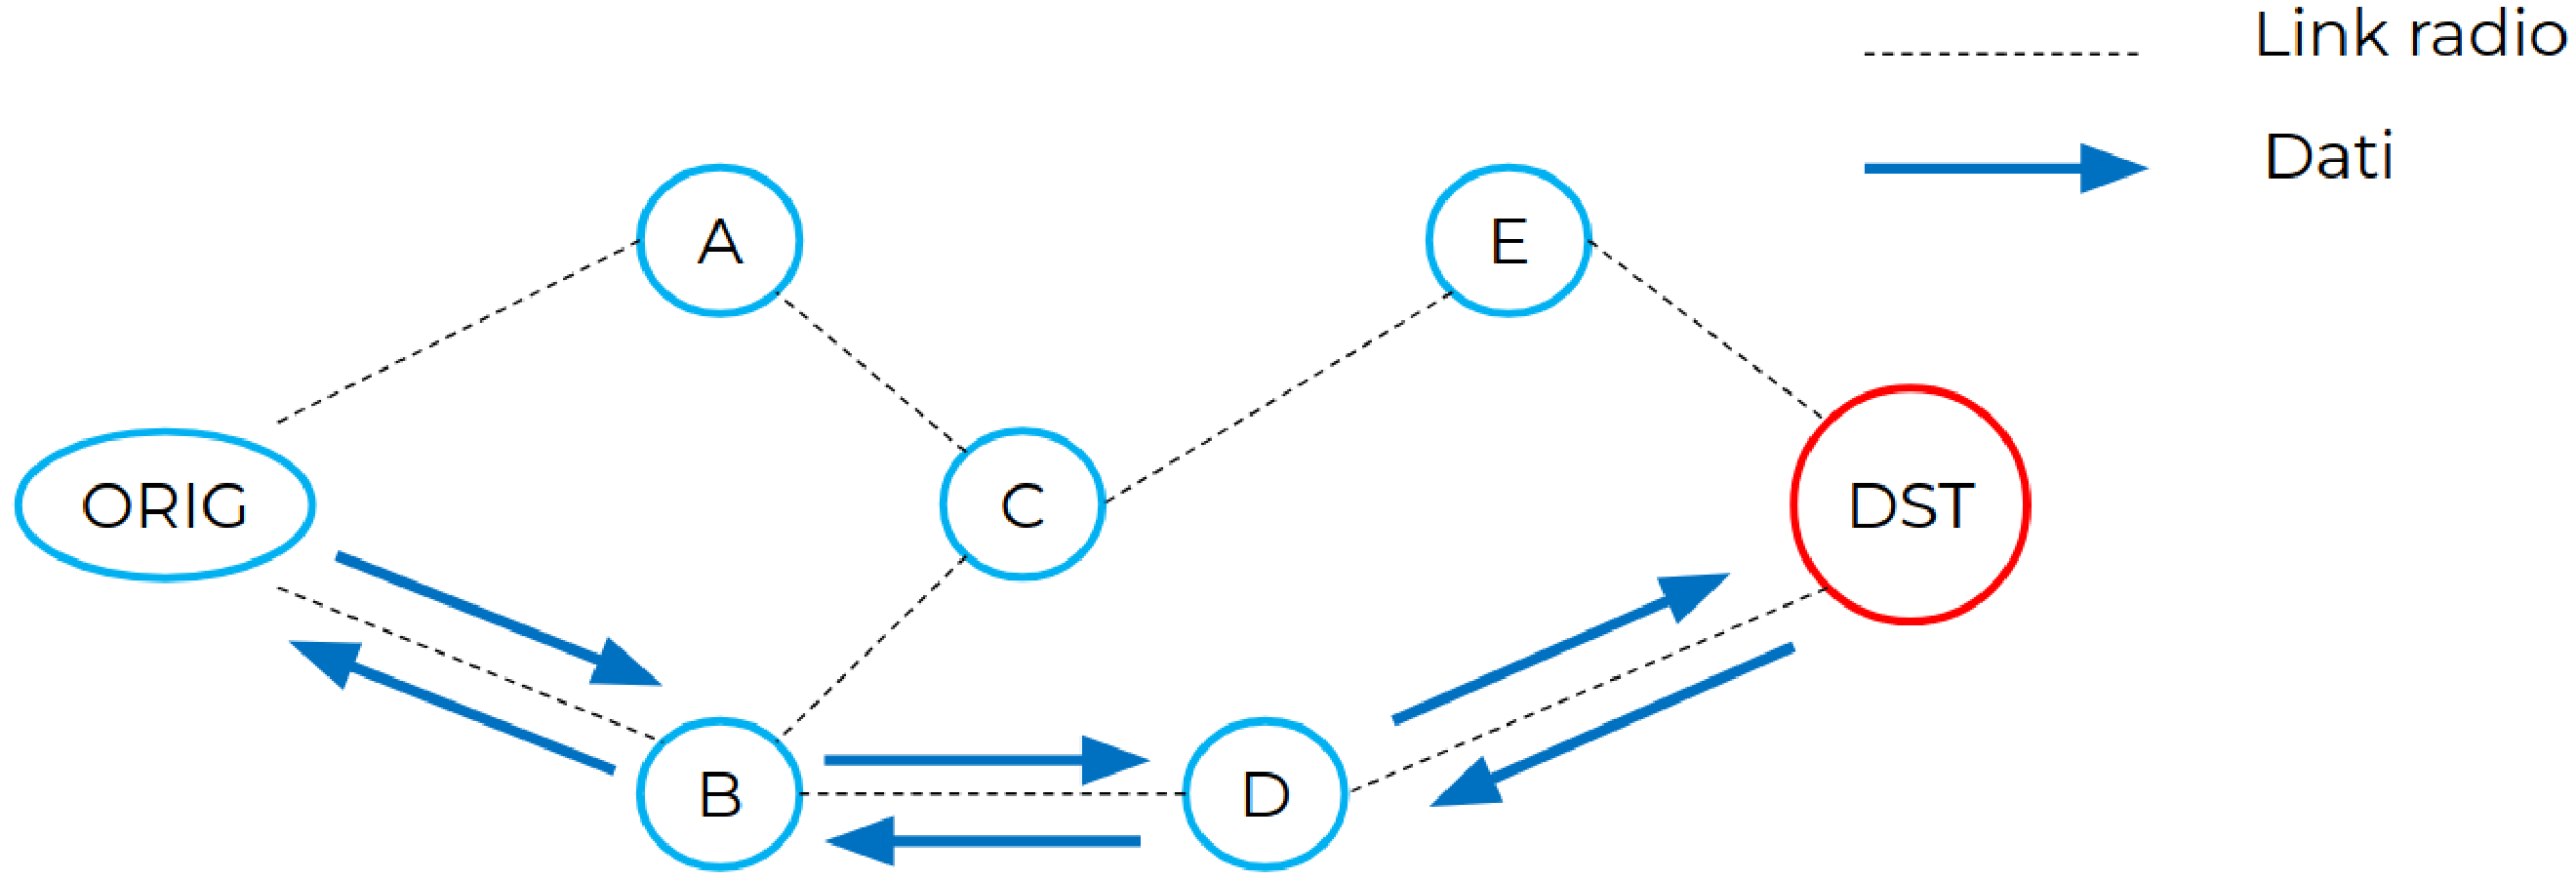
\includegraphics[width=0.9\linewidth]{img/aodv/path1}
\end{center}

\paragraph{Route Request:} I percorsi vengono costruiti tramite \textbf{Route Request RREQ}, sono pacchetti di controllo che permettono di chiedere la costruzione di un percorso verso la destinazione. Non sapendo niente, i messaggi RREQ vengono inviati in broadcast "controllato" (senza loop, il broadcast è fatto a livello IP, con l'indirizzo IP di broadcast). Ogni nodo inoltra RREQ e tiene traccia della provenienza.\\

\paragraph{Route Reply:} La destinazione richiesta in una RREQ risponde in unicast con un messaggio \textbf{Route Reply RREP}.
\begin{center}
	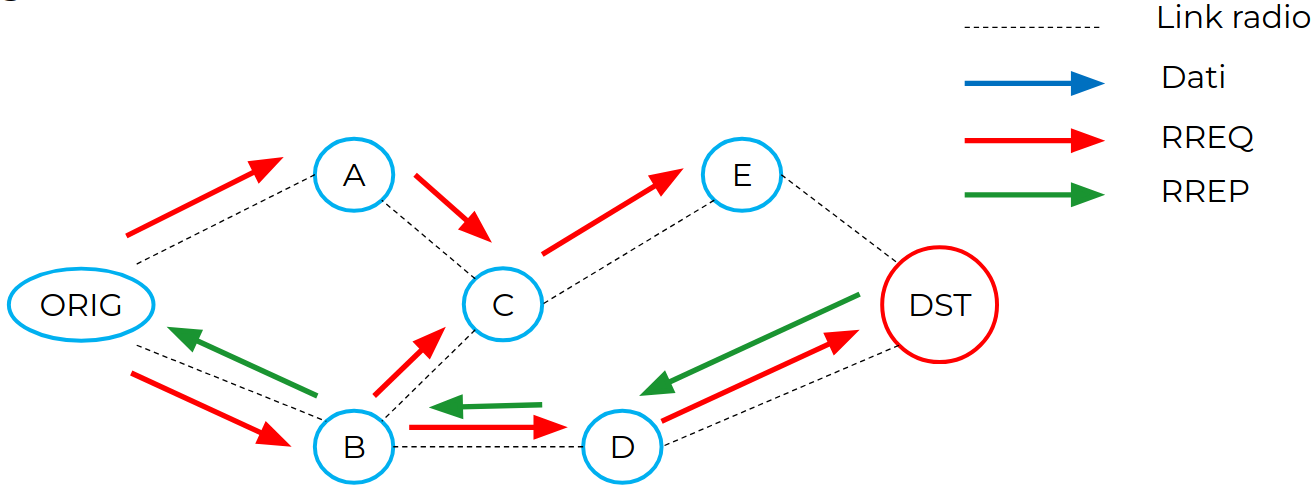
\includegraphics[width=0.9\linewidth]{img/aodv/path2}
\end{center}

La destinazione manda la risposta RREP solo alla prima RREQ (con lo stesso identificatore) ricevuta, in modo da evitare risposte duplicate e trovando (circa) il percorso più breve, dato che risponderà solo al messaggio che ci ha impiegato meno tempo (il primo arrivato).\\

Anche un nodo intermedio può fornire la risposta (inviare il RREP), se conosce l'informazione (sa come arrivare a destinazione) ed è abbastanza "fresca" (lo ha saputo di recente).\\

\paragraph{Route Error:} Un altro messaggio di controllo è \textbf{Route Error RERR}, usato nel caso un link si rompe, per qualsiasi motivo. Il nodo lo invia a tutti i vicini che sa utilizzano quel link per arrivare ad una qualche destinazione.\\

Lo stack è:

\begin{center}
	\renewcommand{\arraystretch}{1.4}
	\begin{tabular}{>{\centering\arraybackslash}m{4cm} | >{\centering\arraybackslash}m{3.5cm} | >{\centering\arraybackslash}m{3.5cm} |}
		\cline{2-3}
		& Messaggi Dati & RREQ/RREP/RERR \\
		\hline
		Livello applicazione & Protocollo\newline applicazione & AODV \\
		\hline
		Livello Trasporto & Trasporto \newline UPD/TCP/\dots & UPD Porta 654 \\
		\hline 
		Livello Rete & \multicolumn{2}{c |}{IP} \\
		\hline
		Livello data link (LL) & \multicolumn{2}{c |}{Ethernet (802.3)/WiFi(802.11)/802.15.4/\dots} \\
		\hline
		Livello fisico (PHY) & \multicolumn{2}{c |}{Ethernet (802.3)/WiFi(802.11)/802.15.4/\dots} \\
		\hline
	\end{tabular}
\end{center}
Quindi i messaggi possono essere dati "normali" tramite TCP oppure i messaggi di controllo AODV. Il livello di rete è IP, mentre i livelli di data link e fisico possono essere uno qualsiasi degli standard IEEE previsti.\\

\subsection{Tabelle di Routing}

Ogni nodo mantiene una tabella delle destinazioni conosciute e l'indicazione del prossimo hop lungo il percorso. Ogni entry in una tabella contiene:
\begin{itemize}
	\item IP destinazione
	\item Sequence number della destinazione
	\item Flag di validità del sequence number della destinazione; permette di disabilitare/abilitare temporaneamente un percorso
	\item Stato del percorso (valido, invalido e altri)
	\item Interfaccia di rete
	\item Hop count, numero di hop per arrivare alla destinazione, ovvero il costo
	\item Lista dei precursori, quali sono i vicini che utilizzano "me" (il nodo) per arrivare a destinazione
	\item Lifetime della entry, ovvero il tempo di scadenza
\end{itemize}

\paragraph{Sequence Number SN:} Tutto cambia in questa rete, quindi ogni entry della tabella possiede un SN che codifica informazioni circa "\textit{la freschezza}" della entry stessa. Il SN è un valore per ogni nodo, ogni possibile destinazione (nodo) ha il proprio e viene modificato esclusivamente dal nodo stesso. \\

Il SN viene incrementato dal nodo in 2 casi: 
\begin{enumerate}
	\item Quando un nodo inizia una ricerca di percorso (RREQ), viene incrementato di 1, previene conflitti con i percorsi inversi stabiliti da una precedente RREQ
	\item Quando un nodo risponde (ovvero il nodo è la destinazione) ad una richiesta di percorso (manda RREP); si aumenta di 1 (solo in alcuni casi in realtà)
\end{enumerate}

Gli altri nodi possono aggiornare il sequence number di una entry in tabella se: 
\begin{itemize}
	\item Il nodo stesso offre un nuovo percorso per se stesso (aggiorna la propria entry nella sua tabella di routing)
	\item Il nodo riceve informazioni più aggiornate per un destinazione
	\item Il percorso verso quella destinazione è scaduto/interrotto
\end{itemize}

Il SN viene confrontato per capire \textit{chi ha l'informazione più aggiornata} per la destinazione. L'incremento viene fatto come se fosse unsigned, il confronto come signed (per gestire overflow).\\

\newpage

\paragraph{RREQ Formato:} Il formato di una RREQ è 
\begin{verbatim}
	 0                   1                   2                   1
	 0 1 2 3 4 5 6 7 8 9 0 1 2 3 4 5 6 7 8 9 0 1 2 3 4 5 6 7 8 9 0 1
	+-+-+-+-+-+-+-+-+-+-+-+-+-+-+-+-+-+-+-+-+-+-+-+-+-+-+-+-+-+-+-+-+
	|     Type      |J|R|G|D|U|   Reserved          |   Hop Count   |
	+-+-+-+-+-+-+-+-+-+-+-+-+-+-+-+-+-+-+-+-+-+-+-+-+-+-+-+-+-+-+-+-+
	|                            RREQ ID                            |
	+-+-+-+-+-+-+-+-+-+-+-+-+-+-+-+-+-+-+-+-+-+-+-+-+-+-+-+-+-+-+-+-+
	|                    Destination IP Address                     |
	+-+-+-+-+-+-+-+-+-+-+-+-+-+-+-+-+-+-+-+-+-+-+-+-+-+-+-+-+-+-+-+-+
	|                  Destination Sequence Number                  |
	+-+-+-+-+-+-+-+-+-+-+-+-+-+-+-+-+-+-+-+-+-+-+-+-+-+-+-+-+-+-+-+-+
	|                     Originator IP Address                     |
	+-+-+-+-+-+-+-+-+-+-+-+-+-+-+-+-+-+-+-+-+-+-+-+-+-+-+-+-+-+-+-+-+
	|                  Originator Sequence Number                   |
	+-+-+-+-+-+-+-+-+-+-+-+-+-+-+-+-+-+-+-+-+-+-+-+-+-+-+-+-+-+-+-+-+
\end{verbatim}

Il \textbf{tipo} è 1, rappresenta il tipo di pacchetto di controllo inviato (RREQ in questo caso).\\

Le \textbf{flag} sono: 
\begin{itemize}
	\item \textbf{\texttt{D}}: Destination Only, solo la destinazione può rispondere, niente nodi intermedi
	\item \textbf{\texttt{U}}: Unknown SN, l'origine non conosce SN della destinazione
	\item \textbf{\texttt{G}}: (Gratuitous) RREP, un nodo intermedio, oltre a rispondere all'origine, deve informare la destinazione della creazione di un percorso (reverse) con l'origine
\end{itemize}

L'\textbf{hop count} viene incrementato di 1 ogni volta che viene inoltrata la RREQ, serve a tenere traccia del "costo" del percorso, in realtà la destinazione vuole rispondere alla RREQ con hop count minore.\\

Il \textbf{RREQ ID} è l'identificativo della richiesta, generato dall'origine e mai modificato, serve a riconoscere la richiesta e le sue copie come un'unica richiesta all'interno della rete.\\

\newpage

Il \textbf{Destination IP Address} è l'indirizzo della destinazione ed il SN indicato è l'ultimo conosciuto (o nessuno nel caso il flag \texttt{U} sia alzato). Se un nodo intermedio ha informazioni riguardo alla destinazione, ma con SN inferiore rispetto a quello indicato, sicuramente l'informazione è troppo vecchia quindi non la invia.\\

\textbf{Originator IP Address} e \textbf{SN} sono le informazioni riguardo l'originator, con il SN più recente inviato.\\

\paragraph{RREQ Creation:} Una RREQ viene creata \textit{quando serve}, ovvero quando un nodo non conosce la destinazione o se la entry è scaduta. Per inviare:
\begin{itemize}
	\item Incremento RREQ ID e il proprio SN (dell'originator)
	\item Se la destinazione è sconosciuta, flag \texttt{U}$=1$
	\item Mantiene una copia di Origine IP, RREQ ID per un tempo denominato \texttt{PATH\_DISCOVERY\_TIME}, definito nello standard, per evitare il riprocessamento e il reinvio dei pacchetto che può essere ricevuto dai vicini
\end{itemize}

\subsubsection{Expanding Ring Search}

 Vogliamo evitare di propagare "inutilmente" una RREQ in tutta la rete, magari la destinazione è vicina. Il TTL dell'header IP viene usato per impostare il massimo numero di hop che una RREQ può fare.\\

Si hanno dei parametri:
\begin{itemize}
	\item \textbf{\texttt{TTL\_START}}: parametro TTL per la prima richiesta
	\item \textbf{\texttt{TTL\_INCREMENT}}: incremento del TTL ad ogni tentativo
	\item \texttt{\textbf{NET\_DIAMETER}}: massimo valore del TTL
\end{itemize}

La request viene fatta inizialmente con un TTL basso, se dopo una certa quantità di tempo il nodo non riceve risposta viene aumentato il TTL ed effettuata una nuova richiesta ("bah, magari è più lontana, ci riprovo"). Ripete fino al TTL massimo. Si espande "l'anello" in cui cercare la destinazione.\\

Questo era \textit{senza conoscenze a priori}, se sono presenti delle conoscenze riguardo un percorso verso la destinazione (scaduto o interrotto) uso la distanza nota in precedenza per iniziare a inviare RREQ. Se ho un'informazione vecchia: parto dalla distanza "vecchia" come TTL. Questo è uno dei motivi per cui non "buttare" subito le informazioni vecchie, vengono tenute per "\textit{un po'}" (definito dallo standard).\\

\paragraph{Retry Policy:} L'origine può riprovare ad inviare RREQ se il primo tentativo non è andato a buon fine. \texttt{\textbf{RREQ\_RETRIES}} è il parametro. Ad ogni nuovo tentativo si incrementano RREQ\_ID e SN.\\

\subsubsection{RREQ Processamento e Inoltro}

Quando un nodo riceve un messaggio RREQ:
\begin{itemize}
	\item Controlla REQ\_ID e Originator IP sono già presenti (già conosciute), se uguali all'ultimo ricevuto entro \texttt{PATH\_DISCOVERY\_TIME} scarto il messaggio
	\item Aggiorno il percorso "reverse", verso originator; ricevendo una RREQ posso capire come arrivare all'origine:
	\begin{enumerate}
		\item Confronto Orig SN (in RREQ) e SN che ho nella tabella, se è maggiore lo aggiorno (potrebbe essere minore, magari la richiesta è molto vecchia, ha fatto giri strani)
		\item Segno la entry come valida (può essere scaduta nel frattempo)
		\item Aggiorno/aggiungo la entry impostando come "next hop" verso orig, il nodo da cui è arrivata la RREQ
		\item Il campo Hop Count della entry viene messo pari al hop count della RREQ (quanto ci ha messo ad arrivare al nodo)
	\end{enumerate}
\end{itemize}

%End L13